\chapter{Uncertainty, Time Evolution, and the Classical Limit}

This lecture unfolds in two large movements. It begins with a brief but purposeful detour about negative energy, then rebuilds the wave-function language needed for the uncertainty principle, proves that principle in a stripped-down but revealing form, and only after that returns to the Schr\"odinger equation itself. The order is part of the argument. These notes follow Leonard Susskind's lecture closely, and where the blackboard organization matters the preserved board evidence kept by LazyingArt LLC and Video2Book is retained alongside the cleaned mathematics.

\section{A Brief Detour: Negative Energy and Dirac's Idea}

Susskind opens by returning to the toy Hamiltonian
\begin{equation}
H=cP.
\end{equation}
For a momentum eigenstate the wave function is a plane wave,
\begin{equation}
\psi_p(x)=e^{ipx}.
\end{equation}
Nothing in the mathematics prefers positive \(p\) to negative \(p\). Both signs give perfectly acceptable waves. But with \(H=cP\), the sign of \(p\) is also the sign of the energy, and that is where the trouble starts.

If negative-energy particles existed in ordinary empty space, then empty space would not be the state of lowest energy. We could always lower the energy further by producing negative-energy particles while compensating with positive-energy radiation. In that world the vacuum would be unstable. So the puzzle is not merely that negative energy is aesthetically unpleasant. It would make the whole world unstable.

The lecture resolves this only qualitatively, and only as an aside. Dirac's move works for fermions: if every negative-energy state is already occupied, Pauli exclusion prevents us from adding more particles to the same states. In that sense the true vacuum is not empty space at all, but a completely filled sea of negative-energy fermion states. The same move fails for bosons, since bosons can pile into one state without limit. So the model is tolerable as a baby version of a fermionic theory, but not as a bosonic one.

That is as far as the lecture wants to go. Susskind explicitly withdraws from the detour and reminds the audience that the course has mostly treated the foundations of quantum mechanics and only the simplest systems. He even jokes that a course in quantum mechanics that never reaches the harmonic oscillator is a disgrace. That self-conscious pause matters. It resets the discussion and prepares the turn back to the actual topic of the day: the Schr\"odinger equation, approached through the wave function.

\section{Wave Functions, Representations, and Many Coordinates}

The wave function is the bridge between the abstract formalism developed earlier and the concrete dynamics Susskind now wants to discuss. In position space we write
\begin{equation}
\psi(x)=\langle x|\psi\rangle,
\end{equation}
the amplitude that the state \(|\psi\rangle\) be found at the position \(x\). The same state can be represented in momentum space by
\begin{equation}
\tilde{\psi}(p)=\langle p|\psi\rangle.
\end{equation}
These are not two different states; they are two descriptions of the same state in two different bases.

The relation between them is a Fourier transform. In the one-dimensional setting of the lecture we may write
\begin{equation}
\psi(x)=\frac{1}{\sqrt{2\pi}}\int dp\,\tilde{\psi}(p)e^{ipx},
\end{equation}
and, conversely,
\begin{equation}
\tilde{\psi}(p)=\frac{1}{\sqrt{2\pi}}\int dx\,\psi(x)e^{-ipx}.
\end{equation}
Susskind does not linger over conventions here. What matters for the lecture is the structural fact that position and momentum descriptions are Fourier-conjugate.

He then briefly broadens the setting. If a particle can move in more than one spatial direction, then its position is described by several coordinates. The crucial point is that those coordinates commute. Susskind pauses to say that this is not a formal inevitability deduced from earlier rules; it is an empirical fact about the way quantum mechanics matches experiment. Thus in more than one dimension the wave function depends on all the commuting coordinates at once.

For several particles, the same idea becomes more dramatic. The wave function is no longer a function of one coordinate but of all the coordinates of all the particles:
\begin{equation}
\psi=\psi(x_1,x_2,\dots,x_N)
\end{equation}
in the one-dimensional many-particle case, or of all components of all particle positions in higher dimensions. One may also use mixed representations, leaving some variables in coordinate space and others in momentum space. But the lecture now deliberately narrows again to one-dimensional motion, where the main ideas can be exposed clearly.

\section{From Noncommutation to a Definition of Uncertainty}

Susskind first states the uncertainty principle in its primitive form. Position and momentum do not commute, so there are no simultaneous sharp eigenstates of both. Position eigenstates are tightly localized in space; momentum eigenstates are plane waves spread over all of space. If one knows position sharply, one is very far from knowing momentum sharply, and vice versa.

He then adds a more qualitative Fourier-transform version of the same point. If we build one representation from the other by Fourier transform, we quickly discover that a narrow function in \(x\) produces a broad function in \(p\), while a narrow function in \(p\) produces a broad function in \(x\). This is already enough to see why the uncertainty principle should exist, but not yet enough to prove a theorem.

The lecture therefore asks a more basic question: what do we mean by uncertainty?

\subsection{Question \& Answer}

Why does the lecture begin by shifting the origin until \(\langle X\rangle=0\)? Because we are not trying to measure where the packet sits; we are trying to measure how wide it is. The center of a distribution can be moved by a harmless change of coordinates. Once the center is placed at the origin, the remaining quantity \(\langle X^2\rangle\) measures spread rather than location.

\begin{definition}
After shifting the origin so that \(\langle X\rangle=0\), we define the squared uncertainty in position by
\begin{equation}
(\Delta x)^2=\langle X^2\rangle.
\end{equation}
If we do not shift the origin, the more general formula is the variance
\begin{equation}
(\Delta x)^2=\langle X^2\rangle-\langle X\rangle^2.
\end{equation}
\end{definition}

In position space the first form becomes
\begin{equation}
(\Delta x)^2=\int dx\,\psi^*(x)\psi(x)\,x^2.
\end{equation}
That is the definition Susskind writes on the board. The farther probability is spread from the chosen origin, the larger \(\langle X^2\rangle\) becomes.

\begin{figure}
\centering

\includegraphics[width=0.78\textwidth]{lecture_10_figure_02.png}
\caption{Position uncertainty defined as an integral over probability density.}
\end{figure}

\begin{figure}
\centering
\begin{tikzpicture}[x=1cm,y=1cm]
\draw[->] (-4.1,0) -- (4.1,0);
\draw[->] (0,0) -- (0,2.5);
\draw[smooth] plot coordinates {(-3.5,0.03) (-2.8,0.10) (-2.0,0.35) (-1.3,0.95) (-0.8,1.55) (-0.3,2.00) (0,2.15) (0.3,2.00) (0.8,1.55) (1.3,0.95) (2.0,0.35) (2.8,0.10) (3.5,0.03)};
\draw[dashed] (0,0) -- (0,2.15);
\node at (0,-0.35) {\(x=0\)};
\node at (2.7,2.05) {\(|\psi(x)|^2\)};
\end{tikzpicture}
\caption{A wave packet after shifting the origin so that its center lies at \(\langle X\rangle=0\).}
\end{figure}

Momentum uncertainty is defined in the same spirit. In momentum space one may write
\begin{equation}
(\Delta p)^2=\int dp\,|\tilde{\psi}(p)|^2\,p^2
\end{equation}
after shifting so that \(\langle P\rangle=0\). But Susskind immediately decides not to use that formula in the proof. Instead he rewrites \((\Delta p)^2\) in the position representation, so that both uncertainties can be handled in one common language.

\section{Proving the Uncertainty Principle}

The lecture now turns deliberately from definition to proof. We first recall how the momentum operator acts in the \(x\)-representation:
\begin{equation}
P=-i\,\partial_x,
\qquad
P^2=-\partial_x^2.
\end{equation}
Therefore
\begin{equation}
(\Delta p)^2=\langle \psi|P^2|\psi\rangle
=
-\int dx\,\psi^*(x)\,\partial_x^2\psi(x).
\end{equation}

\subsection{Question \& Answer}

How can \((\Delta p)^2\) stay positive if the first \(x\)-space formula carries a minus sign? Because the integral itself is negative. The repair is integration by parts, and Susskind slows down to re-teach the rule because he is about to use it repeatedly:
\begin{equation}
\int f\,g'\,dx=-\int f' g\,dx,
\end{equation}
provided the boundary term vanishes.

For a normalized wave function, the boundary term does vanish, and one integration by parts gives
\begin{equation}
(\Delta p)^2
=
\int dx\,(\partial_x\psi^*)(\partial_x\psi),
\end{equation}
which is manifestly real and nonnegative.

The board layout at this stage is important enough to keep. It shows exactly how the lecture has arranged the proof: the two variances on one side, the inequality on the other.

\begin{figure}
\centering

\includegraphics[width=0.88\textwidth]{lecture_10_figure_03.png}
\caption{Variance formulas beside the vector-space inequality.}
\end{figure}

The corresponding cleaned reconstruction is
\begin{align}
(\Delta x)^2 &= \langle \psi|X^2|\psi\rangle, \\
(\Delta p)^2 &= \langle \psi|P^2|\psi\rangle
= \int dx\,(\partial_x\psi^*)(\partial_x\psi), \\
\langle A|A\rangle\,\langle B|B\rangle &\ge |\langle A|B\rangle|^2.
\end{align}

Susskind calls the last relation the triangle inequality in vector-space language. In polished Hilbert-space form it is the Cauchy-Schwarz inequality. But the pedagogical point is the same: we need a general inequality that relates two positive norms to an inner product.

\begin{figure}
\centering
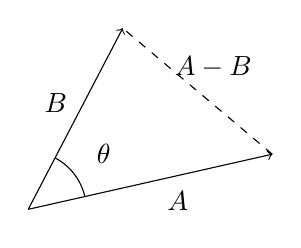
\begin{tikzpicture}[x=1cm,y=1cm]
\draw[->] (0,0) -- (3.1,0.7);
\draw[->] (0,0) -- (1.2,2.3);
\draw[dashed] (3.1,0.7) -- (1.2,2.3);
\node at (1.9,0.1) {\(A\)};
\node at (0.35,1.35) {\(B\)};
\node at (2.35,1.8) {\(A-B\)};
\draw (0.72,0.16) arc[start angle=13,end angle=62,radius=0.75];
\node at (0.96,0.70) {\(\theta\)};
\end{tikzpicture}
\caption{The geometric picture behind the inequality Susskind invokes.}
\end{figure}

Now comes the real trick. We choose vectors so that their norms are exactly the uncertainties we are trying to relate:
\begin{equation}
|A\rangle=X|\psi\rangle,
\qquad
|B\rangle=P|\psi\rangle.
\end{equation}
In the \(x\)-representation these become
\begin{equation}
A(x)=x\psi(x),
\qquad
B(x)=-i\,\frac{d\psi}{dx}.
\end{equation}
And the corresponding inner product is
\begin{equation}
|\langle A|B\rangle|^2
=
\left|
\int dx\,\psi(x)\,x\,\frac{d\psi}{dx}
\right|^2
\end{equation}
up to the harmless overall phase that disappears inside the absolute value.

\begin{figure}
\centering

\includegraphics[width=0.84\textwidth]{lecture_10_figure_04.png}
\caption{Auxiliary states \(A\) and \(B\) in the uncertainty proof.}
\end{figure}

The lecture now introduces one more simplification. To avoid a blackboard full of \(\psi^*\)'s, Susskind assumes that \(\psi(x)\) is real. He explicitly says this is only a pedagogical simplification, not the general theorem. We follow him here.

\begin{theorem}
In the simplified proof where \(\langle X\rangle=\langle P\rangle=0\), \(\psi(x)\) is taken real, and \(\hbar=1\), one finds
\begin{equation}
\Delta x\,\Delta p\ge \frac{1}{2}.
\end{equation}
\end{theorem}

\begin{proof}
By construction,
\begin{equation}
\langle A|A\rangle=(\Delta x)^2,
\qquad
\langle B|B\rangle=(\Delta p)^2.
\end{equation}
Cauchy-Schwarz therefore gives
\begin{equation}
(\Delta x)^2(\Delta p)^2\ge |\langle A|B\rangle|^2.
\end{equation}
Now, because \(\psi\) is real,
\begin{equation}
\psi\,\frac{d\psi}{dx}
=
\frac{1}{2}\frac{d}{dx}(\psi^2).
\end{equation}
So
\begin{equation}
\langle A|B\rangle
\sim
\int dx\,x\,\psi\,\frac{d\psi}{dx}
=
\frac{1}{2}\int dx\,x\,\frac{d}{dx}(\psi^2),
\end{equation}
where the omitted phase is irrelevant once we take the absolute value.

Integrating by parts gives
\begin{equation}
\frac{1}{2}\int dx\,x\,\frac{d}{dx}(\psi^2)
=
-\frac{1}{2}\int dx\,\psi^2,
\end{equation}
since the boundary term vanishes and \(\partial_x x = 1\). For a normalized wave function,
\begin{equation}
\int dx\,\psi^2=1.
\end{equation}
Therefore
\begin{equation}
|\langle A|B\rangle|^2=\frac{1}{4},
\end{equation}
and hence
\begin{equation}
(\Delta x)^2(\Delta p)^2\ge \frac{1}{4}.
\end{equation}
Taking square roots,
\begin{equation}
\Delta x\,\Delta p\ge \frac{1}{2}.
\end{equation}
When the factors of \(\hbar\) are restored, this becomes
\begin{equation}
\Delta x\,\Delta p\ge \frac{\hbar}{2}.
\end{equation}
\end{proof}

\begin{figure}
\centering

\includegraphics[width=0.84\textwidth]{lecture_10_figure_05.png}
\caption{The boxed uncertainty bound as it appears on the board.}
\end{figure}

The cleaned final form, correcting the board's strict sign, is
\begin{equation}
\Delta x\,\Delta p\ge \frac{1}{2}
\end{equation}
in units with \(\hbar=1\), and
\begin{equation}
\Delta x\,\Delta p\ge \frac{\hbar}{2}
\end{equation}
when dimensions are restored.

\subsection{Question \& Answer}

Why is the final statement really \(\ge\), and when can equality occur? Susskind is corrected on exactly this point during the lecture, and he immediately agrees that it matters. If the inequality were not sharp, perhaps a stronger one could still be proved. But in fact equality is attainable. There are wave packets for which
\begin{equation}
\Delta x\,\Delta p=\frac{\hbar}{2},
\end{equation}
and those are precisely the minimal uncertainty packets that the next lecture will study.

\section{After the Proof: Minimal Packets and Other Conjugate Pairs}

The lecture does not drop the uncertainty principle the moment the theorem is written down. It lingers on the live pressure points that the proof has raised.

First, the integration-by-parts rule really does depend on the boundary term vanishing. For normalizable states that condition is natural: \(\psi(x)\) must decay so that \(\int |\psi|^2 dx\) is finite. The theorem is not independent of that structure.

Second, equality matters. The existence of minimal packets means the inequality is tight. We have not simply proved some loose lower bound.

\subsection{Question \& Answer}

Does the same kind of argument apply to time and energy? Susskind answers yes, but more cautiously than in the position-momentum case. The relation is again Fourier-theoretic, but its use is subtler. The time dependence of a state may be written schematically as
\begin{equation}
|\psi(t)\rangle=\int dE\,\phi(E)e^{-iEt}|E\rangle.
\end{equation}
Thus time and energy are related in the same broad Fourier sense as position and momentum. If a wave packet passes an observer during a very short time interval, the corresponding energy spread must be broad; if the energy spread is very narrow, the time of passage is correspondingly uncertain. The lecture does not attempt a full formal treatment here, and neither should we.

The same broad pattern extends to other conjugate pairs. A rigid body described by an angle \(\theta\) has angular momentum conjugate to that angle, and one again finds an uncertainty relation of the same family. These remarks are brief in the lecture, but they are important. They tell us that the position-momentum theorem is one instance of a larger structure.

\section{The Schr\"odinger Equation in Abstract and in Position Space}

Only after the uncertainty discussion has run its course does Susskind say, in effect, let us return to the Schr\"odinger equation. He re-enters through the abstract law of time evolution,
\begin{equation}
i\,\frac{d}{dt}|\psi\rangle=H|\psi\rangle.
\end{equation}
The left-hand side of the board frame is partly cropped, but the transcript makes the intended equation unmistakable.

He then chooses the standard Hamiltonian for a particle in a potential,
\begin{equation}
H=\frac{P^2}{2m}+V(X).
\end{equation}
This is exactly the classical particle Hamiltonian, now elevated to operator form. The lecture is quite frank about the logic: one takes the classical Hamiltonian, quantizes it, and then asks whether the resulting wave-packet motion reproduces classical mechanics in the circumstances where classical mechanics ought to work.

\begin{figure}
\centering

\includegraphics[width=0.76\textwidth]{lecture_10_figure_06.png}
\caption{The board reset as the lecture returns to abstract time evolution.}
\end{figure}

In the \(x\)-representation we replace \(P\) by \(-i\partial_x\), and so
\begin{equation}
i\,\partial_t\psi(x,t)
=
-\frac{1}{2m}\partial_x^2\psi(x,t)+V(x)\psi(x,t).
\end{equation}
It is convenient, and faithful to the lecture, to also write the complex-conjugate equation:
\begin{equation}
\partial_t\psi^*(x,t)
=
-\frac{i}{2m}\partial_x^2\psi^*(x,t)+iV(x)\psi^*(x,t).
\end{equation}

\subsection{Question \& Answer}

What does it mean for \(V(x)\) to be an operator? In this representation the answer is simple: it multiplies the wave function. The operator \(X\) multiplies by \(x\); a function of \(X\) multiplies by the corresponding function. Thus
\begin{equation}
V(X)\psi(x)=V(x)\psi(x).
\end{equation}
Susskind pauses over this because it is a definition, and definitions in physics have to earn their keep. The payoff will come when we see what this choice implies for the motion of expectation values.

\section{Expectation Values, Ehrenfest-Type Equations, and the Limits of Classical Motion}

The lecture's final aim is to connect wave-packet motion to classical motion. If the packet remains sufficiently coherent and localized, then its center may be identified with the expectation value of position. We therefore ask how \(\langle X\rangle\) and \(\langle P\rangle\) change with time.

\begin{proposition}
For the Hamiltonian \(H=\frac{P^2}{2m}+V(X)\),
\begin{equation}
\frac{d}{dt}\langle X\rangle=\frac{\langle P\rangle}{m}.
\end{equation}
\end{proposition}

\begin{proof}
Start from
\begin{equation}
\langle X\rangle=\int dx\,\psi^*(x,t)\,x\,\psi(x,t).
\end{equation}
Differentiating gives
\begin{equation}
\frac{d}{dt}\langle X\rangle
=
\int dx\,(\partial_t\psi^*)x\psi
+
\int dx\,\psi^*x(\partial_t\psi).
\end{equation}
Substitute the Schr\"odinger equations for \(\partial_t\psi\) and \(\partial_t\psi^*\). The two terms involving \(V(x)\) cancel exactly, since they are equal and opposite. What remains is
\begin{equation}
\frac{d}{dt}\langle X\rangle
=
\frac{i}{2m}\int dx\,
\left[
-(\partial_x^2\psi^*)x\psi+\psi^*x(\partial_x^2\psi)
\right].
\end{equation}
Now integrate by parts. This is the move the lecture returns to again and again. After one integration by parts on each term, the pieces involving \(x\,(\partial_x\psi^*)(\partial_x\psi)\) cancel, and we are left with
\begin{equation}
\frac{d}{dt}\langle X\rangle
=
\frac{i}{2m}\int dx\,
\left[
(\partial_x\psi^*)\psi-\psi^*(\partial_x\psi)
\right].
\end{equation}
Since \(\langle P\rangle\) is real, this is precisely
\begin{equation}
\frac{d}{dt}\langle X\rangle
=
\frac{1}{m}\int dx\,\psi^*(-i\partial_x)\psi
=
\frac{\langle P\rangle}{m}.
\end{equation}
\end{proof}

This is the first half of mechanics: momentum divided by mass is velocity. Susskind pauses over the point that no localization assumption has yet been used. The relation is exact.

\begin{proposition}
For the same Hamiltonian,
\begin{equation}
\frac{d}{dt}\langle P\rangle=-\left\langle \frac{dV}{dx}\right\rangle.
\end{equation}
\end{proposition}

\begin{proof}
Write
\begin{equation}
\langle P\rangle
=
\int dx\,\psi^*(-i\partial_x)\psi.
\end{equation}
Differentiating with respect to time gives
\begin{equation}
\frac{d}{dt}\langle P\rangle
=
-i\int dx\,(\partial_t\psi^*)\,\partial_x\psi
-i\int dx\,\psi^*\,\partial_x(\partial_t\psi).
\end{equation}
Integrate the second term by parts:
\begin{equation}
\frac{d}{dt}\langle P\rangle
=
-i\int dx\,(\partial_t\psi^*)\,\partial_x\psi
+i\int dx\,(\partial_x\psi^*)\,\partial_t\psi.
\end{equation}
Now substitute the Schr\"odinger equations. The kinetic pieces combine into a total derivative,
\begin{equation}
-\frac{1}{2m}\int dx\,\partial_x\!\left[(\partial_x\psi^*)(\partial_x\psi)\right],
\end{equation}
so with vanishing boundary terms they disappear.

The potential terms combine into
\begin{equation}
\int dx\,V(x)\left[\psi^*(\partial_x\psi)+(\partial_x\psi^*)\psi\right].
\end{equation}
But the bracket is just the derivative of the probability density:
\begin{equation}
\psi^*(\partial_x\psi)+(\partial_x\psi^*)\psi
=
\partial_x(\psi^*\psi).
\end{equation}
Therefore
\begin{equation}
\frac{d}{dt}\langle P\rangle
=
\int dx\,V(x)\,\partial_x(\psi^*\psi).
\end{equation}
One final integration by parts yields
\begin{equation}
\frac{d}{dt}\langle P\rangle
=
-\int dx\,\psi^*(x,t)\psi(x,t)\,\frac{dV}{dx}
=
-\left\langle \frac{dV}{dx}\right\rangle.
\end{equation}
\end{proof}

If we define the force by
\begin{equation}
F(x)=-\frac{dV}{dx},
\end{equation}
then the result reads
\begin{equation}
\frac{d}{dt}\langle P\rangle=\langle F(X)\rangle.
\end{equation}
Again, nothing approximate has been done.

\subsection{Question \& Answer}

If these equations are exact, why are we not already finished with the classical limit? Because the exact result is
\begin{equation}
\frac{d}{dt}\langle P\rangle=\langle F(X)\rangle,
\end{equation}
whereas classical motion of the packet center would require
\begin{equation}
\frac{d}{dt}\langle P\rangle\approx F(\langle X\rangle).
\end{equation}
In general those are not the same thing:
\begin{equation}
\langle F(X)\rangle \neq F(\langle X\rangle).
\end{equation}

Susskind gives a beautifully sharp example. Suppose
\begin{equation}
F(x)=x^2,
\end{equation}
and suppose the wave packet consists of two separated bumps, symmetric about the origin. Then
\begin{equation}
\langle X\rangle=0,
\qquad
F(\langle X\rangle)=F(0)=0,
\end{equation}
but
\begin{equation}
\langle F(X)\rangle=\langle X^2\rangle>0.
\end{equation}
So the exact Ehrenfest-type equations do not by themselves produce Newton's law for the center of the packet. A further approximation is needed: the packet must be localized enough that the force is effectively constant across its width.

This is the point at which the lecture returns from algebra to physics. A smooth potential does not disturb a narrow packet very much, and then the packet moves more or less classically. A sharp potential feature, by contrast, tends to break the packet into pieces and scatter them.

Susskind then makes the argument more concrete with an order-of-magnitude estimate. In many reasonable circumstances macroscopic objects nearly saturate the uncertainty relation, so that
\begin{equation}
\Delta x\,\Delta p \sim \hbar.
\end{equation}
Since \(\Delta p=m\,\Delta v\), this becomes
\begin{equation}
\Delta x\,\Delta v \sim \frac{\hbar}{m}.
\end{equation}
This is not a new exact theorem; it is a heuristic estimate. But it captures the point. When \(m\) is large, the positional spread needed for a given velocity spread becomes small. A heavy body therefore tends to carry a tightly concentrated packet. Sharp details of the potential then look broad compared with the packet, and the packet moves through them without being torn apart. When \(m\) is small, the spread is larger, and the same potential is seen as ragged and disruptive.

That is why the lecture ends with a contrast between bowling balls and electrons, and between smooth fields and sharp structures. An electron in a very smooth electric field can move as an almost classical packet. The same electron striking the sharp structure near a nucleus scatters in all directions. The lecture then widens the point once more: photons behave the same way. Smoothly varying media lead to geometric optics; diffraction gratings and other sharp structures spread waves out.

\begin{remark}
Quantum mechanics is not expected to reproduce classical mechanics in every imaginable circumstance. It is expected to reproduce it when packets remain coherent and localized, and when the potential is smooth on the scale seen by those packets.
\end{remark}

\section{Summary}

The lecture proceeds with great deliberateness. It settles one loose conceptual end about negative energy, resets the agenda, rebuilds the wave-function language of position and momentum, and turns the uncertainty principle from a Fourier-transform intuition into a theorem. Only then does it return to the Schr\"odinger equation, derive exact equations for \(\langle X\rangle\) and \(\langle P\rangle\), and finally insert the crucial caveat: exact expectation-value equations are not yet classical mechanics. The classical limit appears only when wave packets stay narrow and potentials stay smooth enough that \(\langle F(X)\rangle\) may be replaced by \(F(\langle X\rangle)\). That final distinction is not an appendix to the lecture. It is the point toward which the entire lecture has been moving.